\documentclass[12pt, twocolumn]{report}
\usepackage{setspace}
\usepackage{geometry}
\usepackage{hyperref}
\usepackage{graphicx}

\onehalfspacing
\geometry{margin=25mm}

\author{Liuchuyao Xu}
\title{General-purpose Computing on Graphics Processing Units for Real-time Analysis of Scanning Electron Microscope Images}

\begin{document}
\maketitle

\begin{abstract}
\end{abstract}

\section{Introduction}
\paragraph{}
The scanning electron microscope (SEM) is a type of microscope that produces images using signals generated from the interaction between electrons and the surface under observation. It has higher resolutions than the traditional optical microscope---an SEM can have a resolution lower than one nanometre, whereas that of an optical microscope is limited to a few hundred nanometres. This has benefited a variety of fields by allowing scientists to see micro-details of objects that were previously impossible to observe. For example, the SEM can be used to study structures of semiconductor devices \cite{SEM for semiconductors} and to view changes in bacterial cells \cite{SEM for baterial cells}.

\paragraph{}
Fig. \ref{SEM basic construction} illustrates how an SEM works. The electron gun generates an electron beam, which is transformed into an electron probe after passing through the condenser lens and objective lens. It is then scanned across the specimen under the effect of the scanning coil. As a result of the interaction between the incident electrons and the specimen, some electrons (which are called secondary electrons) are emitted from the specimen. The detector collects the secondary electrons and generates signals based on their energy levels. The display unit uses the signals to produce one image after each complete scan of the specimen.

\begin{figure}[htbp]
    \centering
    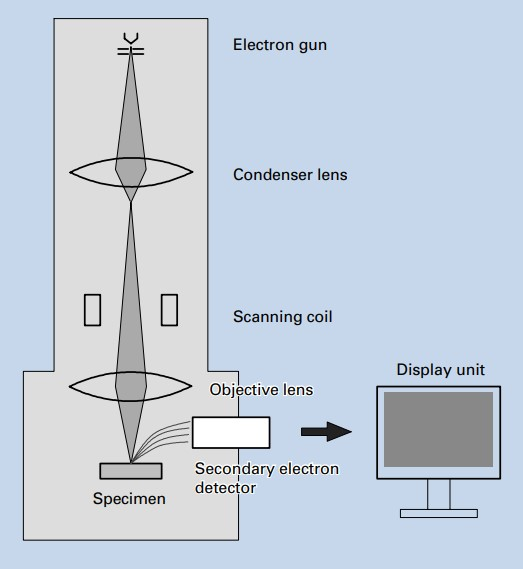
\includegraphics[width=0.45\textwidth]{Figures/SEM basic construction.jpg}
    \caption{Basic construction of an SEM \cite{SEM A to Z}.}
    \label{SEM basic construction}
\end{figure}

\paragraph{}
Many image analysis methods have applications in the field of SEM, and the fast Fourier transform is an especially popular one since it can be used to evaluate the focusing and astigmatism of an SEM [see section TBC]; however, due to the complexity of the algorithm and a lack of fast hardware, real-time analysis had been either impossible or impractical in the past. In 1997, with an advanced central processing unit (CPU)---the Pentium Pro, it was only possible to achieve a refresh rate of 0.6 frames per second for 8-bit 1024 $\times$ 1024 input images \cite{SEM image sharpness measurement}. Although the enhancement of CPUs has enabled faster computations throughout the years, what really brings the speed to a different level is the development of graphics processing units (GPUs).

\paragraph{}
The GPU used to be a highly specialised hardware that was designed to excel in rendering complex, high-resolution, real-time 3D scenes for games; however, its special architecture has made it outperform the CPU in many other areas and resulted in the birth of the idea of general-purpose computing on graphics processing units (GPGPU) \cite{GPU computing}, where the GPU is used to perform computations that are traditionally handled by the CPU.

\paragraph{}
A key characteristic of GPUs is massive parallelism. Depending on their positions, pixels in a 3D scene often require different processing to achieve effects such as lighting, blurring, and fogging. The GPU does this by breaking down the scene into fragments and manipulating each fragment individually. Modern GPUs have thousands of parallel processor cores each running tens of parallel threads to meet the the high requirement for parallelism. For example, the NVIDIA GeForce GTX 1060 has 1280 cores and each of them is capable of running 16 threads; a similarly prices CPU---the Intel i7-7700---has only 4 cores each running 8 threads. It is worth mentioning that the processing cores on a GPU are not as sophisticated as a full CPU and run at a lower clock frequency. The processor clock frequency of the GTX 1060 is 1708 MHz whereas the i7-7700 has a base processor frequency of 3600 MHz. This means that GPGPU is more useful for applications that involve simple, repetitive, parallel tasks. A recent example is deep learning, where computations that follow the same logical sequence of control need to be performed on a deep network of nodes. Typical deep learning networks in 2015 consist of about one million nodes \cite{Deep learning}, which means that the computations cannot be done efficiently on a CPU.

\paragraph{}
This report investigates the performance difference between GPUs and CPUs, and presents a diagnostic tool developed based on GPGPU, which can perform real-time histogram equalisation and FFT on images captured by an SEM. The tool was used to implement an automatic focusing and astigmatism correction algorithm, and the results are discussed.

\section{}

\section{Conclusions}

\begin{thebibliography}{00}
    \bibitem{SEM for semiconductors}
    C. REEVES, ``The uses of scanning electron microscopy for studying semiconductor devices,'' International Journal of Electronics, vol. 77, no. 6, pp. 919-928, 1994, doi: 10.1080/00207219408926111.

    \bibitem{SEM for baterial cells}
    T. Cushnie, N. O’Driscoll and A. Lamb, ``Morphological and ultrastructural changes in bacterial cells as an indicator of antibacterial mechanism of action,'' Cellular and Molecular Life Sciences, vol. 73, no. 23, pp. 4471-4492, 2016, doi: 10.1007/s00018-016-2302-2.

    \bibitem{SEM A to Z}
    ``SEM A to Z,'' Jeol.co.jp, [Online], available: \url{https://www.jeol.co.jp/en/applications/pdf/sm/sem_atoz_all.pdf}. [Accessed: 18 May 2020].

    \bibitem{SEM image sharpness measurement}
    A. Vladár, M. Postek and M. Davidson, ``Image sharpness measurement in scanning electron microscopy-part II,'' Scanning, vol. 20, no. 1, pp. 24-34, 2006, doi: 10.1002/sca.1998.4950200104.

    \bibitem{GPU computing}
    J. D. Owens, M. Houston, D. Luebke, S. Green, J. E. Stone and J. C. Phillips, ``GPU Computing,'' in Proceedings of the IEEE, vol. 96, no. 5, pp. 879-899, May 2008, doi: 10.1109/JPROC.2008.917757.

    \bibitem{Deep learning}
    Ian Goodfellow; Yoshua Bengio; Aaron Courville, ``Deep learning,'' in Deep Learning, The MIT Press, 2017, p. 23.
\end{thebibliography}
\end{document}
